\documentclass[aspectratio=169,usenames,dvipsnames]{beamer}
\beamertemplatenavigationsymbolsempty
% \documentclass{beamer}

% UNCOMMENT FOR HANDOUTS
% \usepackage{pgfpages}
% \pgfpagesuselayout{2 on 1}[landscape,letterpaper,border shrink=5mm]
% \setbeameroption{show notes}

\mode<presentation>
\usetheme{Boadilla}
\usecolortheme{spruce}
\usepackage{../../LizStyle,ulem}
\usepackage{hyperref}
\usepackage{color}
\usepackage[color,matrix,arrow]{xy}
% \input xy
% \xyoption{all}
\usepackage{tikz}
\usepackage{tikz-cd}
\tikzset{commutative diagrams/diagrams={ampersand replacement=\&}}

\AtBeginSection{\frame{\sectionpage}}


\newcommand{\bvfill}{\vskip0pt plus 1filll}

% ==========Command for putting comments and removing them=======
% Visible:
\newcommand{\InstructorNotes}[1]{\textit{\color{orange}#1}}
\newcommand{\InstructorList}[1]{
\begin{itemize}
	\color{orange}
	#1
\end{itemize}
}
% Removed:
\renewcommand{\InstructorNotes}[1]{}
\renewcommand{\InstructorList}[1]{}
\usepackage{multimedia}
\usepackage{graphbox}

% \usepackage{algpseudocode}


\graphicspath{ {Figures/} {../../Figures/} }



\begin{document}
%\pdfoptionpdfminorversion 5
%\logo{\includegraphics[height=1.5cm]{dukeshield.pdf}}
\title[Lec 1]{Intro and First Day Stuff}
\subtitle{Lecture 1 - CMSE 381}
\date{Mon, Jan 12, 2026}



\institute[MSU-CMSE]{Michigan State University\\
			::\\
          Dept of Computational Mathematics, Science \& Engineering}
\author[Dr.~Bao]{Prof.~Lianzhang Bao}

\begin{frame}
 \titlepage


\end{frame}
%--------------------------
%--- Next Frame ---%
\begin{frame}{People in this lecture}

\begin{columns}
	\column{.4\textwidth}
	\centering
\includegraphics[alt={personal photo of Lianzhang Bao},width = .4\textwidth]{Bao}

\textbf{Dr.~Bao }(he/him)\\
Assistant Professor, CMSE, MSU\\

	\column{.4\textwidth}
	\centering
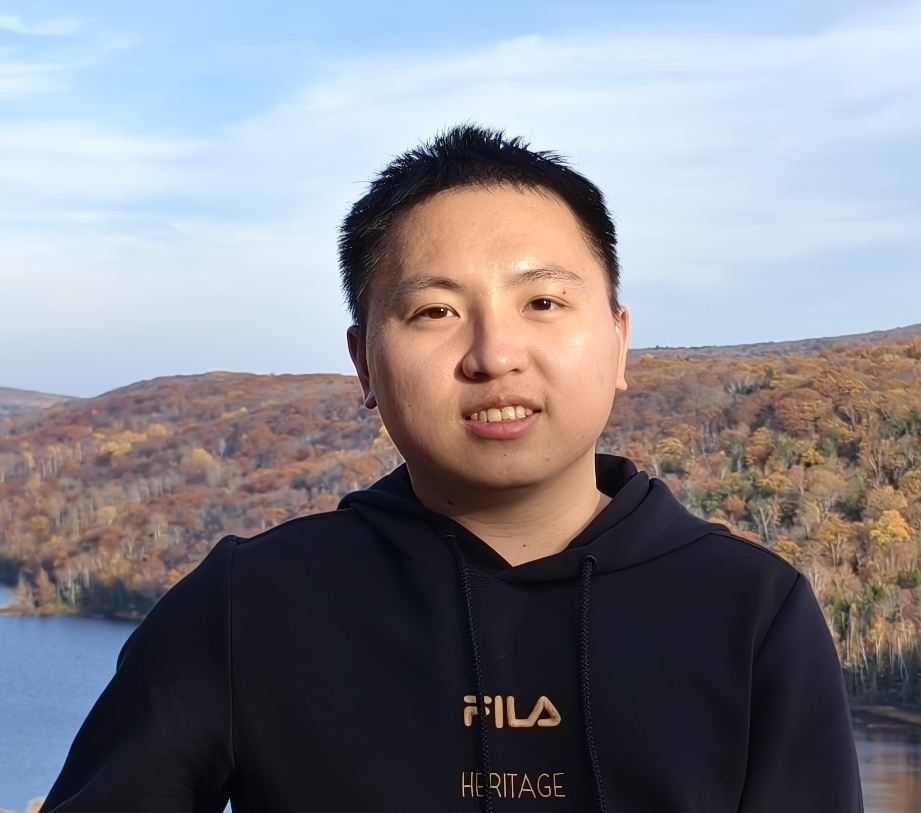
\includegraphics[alt={personal photo of Siyu Guo},width = .55\textwidth]{SiyuGuo.jpeg}

\textbf{Siyu Guo} (He/him)\\
Graduate Student, CMSE, MSU\\
% At MSU since 2020
\end{columns}

\end{frame}
%--- Next Frame ---%
% \begin{frame}[t]{About me}
% 	\centering
% 	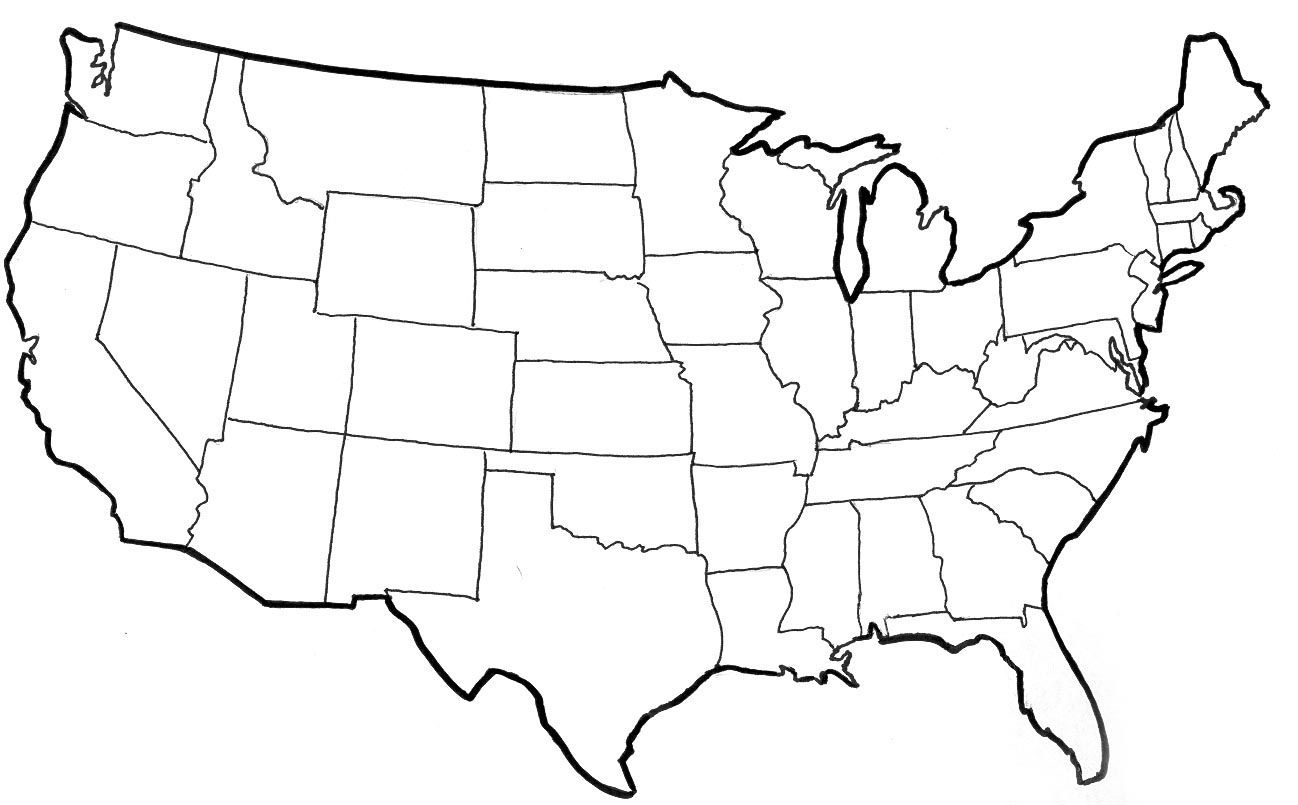
\includegraphics[width = .7\textwidth]{US-state-outline-map}
% \end{frame}
% %--- Next Frame ---%
% \begin{frame}[c]{About you..... Annotate me!}

% \begin{columns}
% \column{.6\textwidth}
% \centering
% 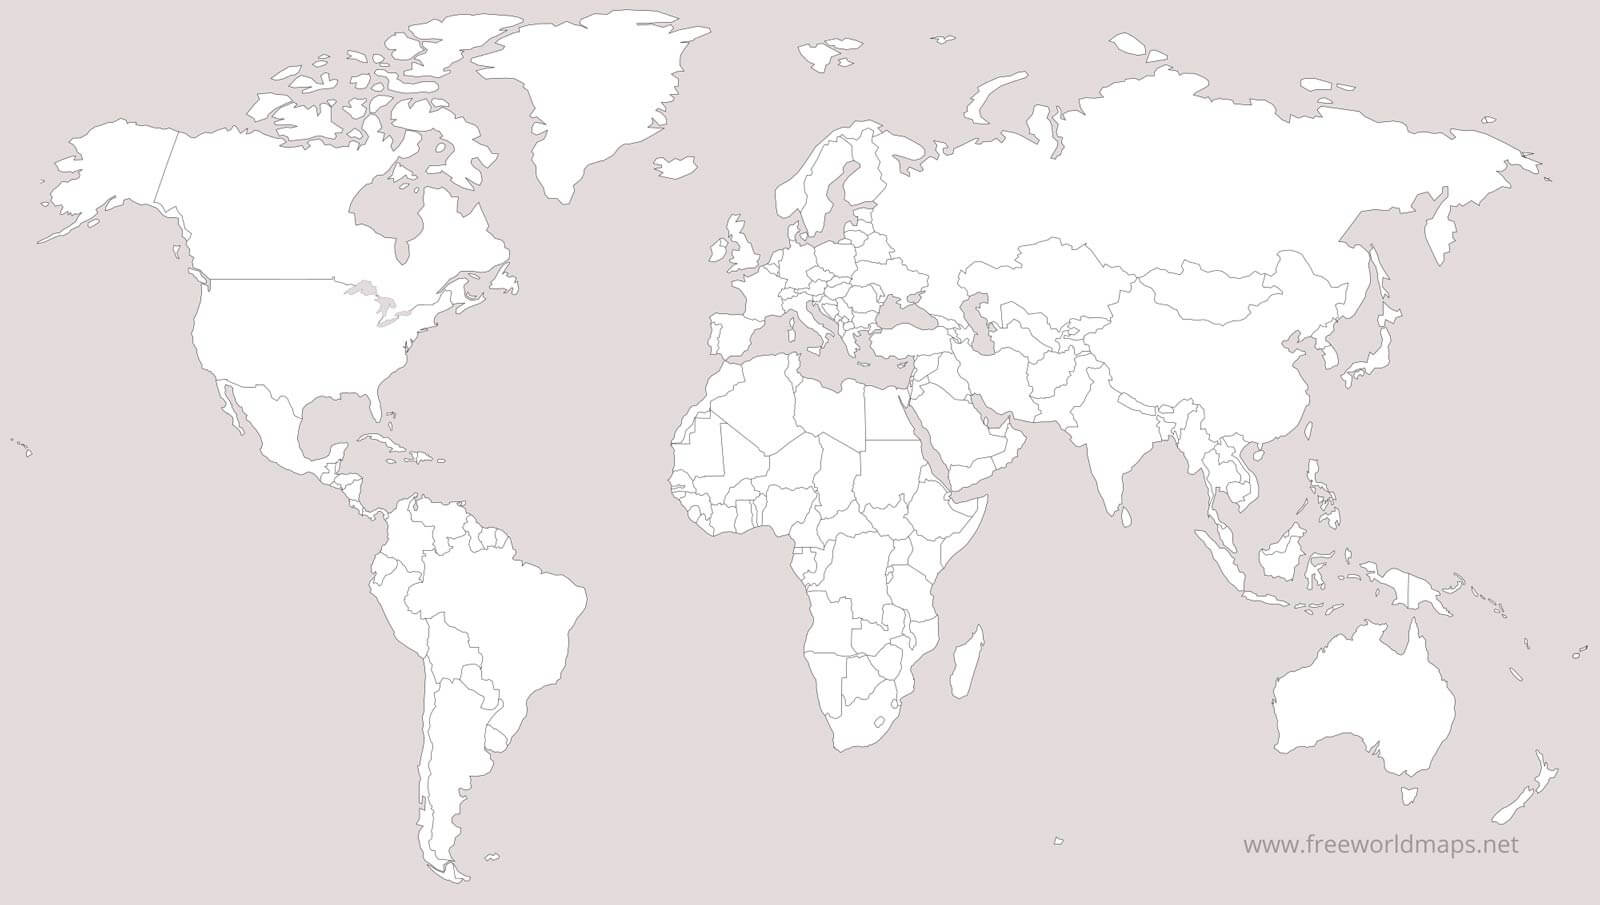
\includegraphics[width = \textwidth]{../Figures/world-outline-map}
% \column{.4\textwidth}
% \centering
% 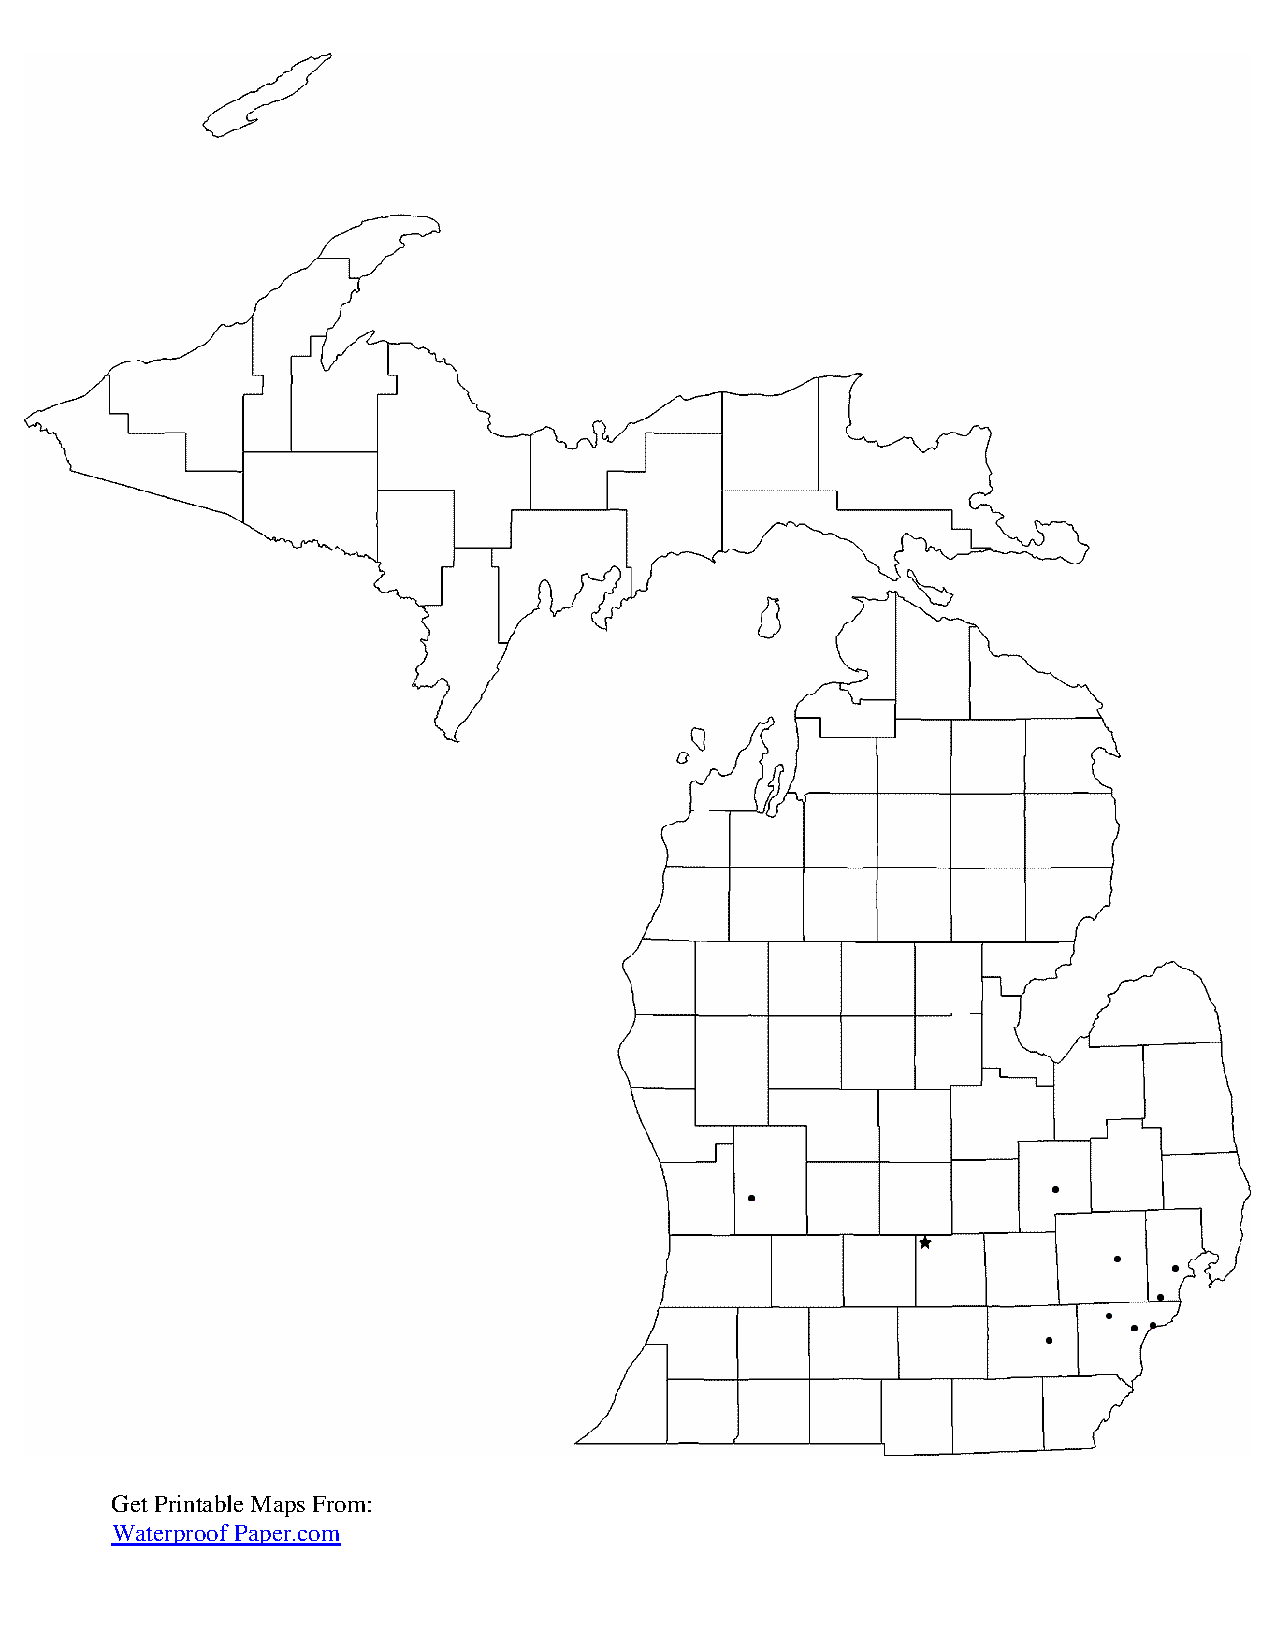
\includegraphics[width = \textwidth]{../Figures/michigan-cities-location-map}
% \end{columns}

% \end{frame}
%--- Next Frame ---%
\begin{frame}[c]{What is this course about?}
	Topics:
	\begin{itemize}
		\item
Fundamental concepts of data science
		\item
Regression
		\item
Classification
		\item
Dimension reduction
		\item
Resampling methods
		\item
Tree-based methods, etc.
	\end{itemize}
\end{frame}
%--- Next Frame ---%
% \begin{frame}[c]{Zoom and etiquette}
% 	\begin{itemize}
% 		\item Online until at least February......
% 		\item
% 	Please ask questions!
% 		\item
% 	Cameras
% 	\item Kids \& Pets
% 	\end{itemize}
% \end{frame}
%--- Next Frame ---%
\begin{frame}{D2L and where to find grades}
	\centering 
	\url{https://d2l.msu.edu/d2l/home/2387930}

\includegraphics[alt={screenshot of course page on D2L},width=.7\textwidth]{D2L_s26_001.png} 
\end{frame}
%--- Next Frame ---%
%\begin{frame}[c]{Slack and where to find announcements/ask questions}
%	\centering
%	Join \texttt{cmse-courses} slack: \url{https://tinyurl.com/cmse-courses-slack-invite}

%	\qquad 

%\includegraphics[width=.7\textwidth]{slack_s26_001.png}


%\end{frame}
%--- Next Frame ---%
\begin{frame}[c]{Course Website and where to find slides and jupyter notebooks}
	\centering
	\url {https://cmse.msu.edu/CMSE381}\\
	--or--\\
	\url{https://msu-cmse-courses.github.io/CMSE381-S26/}
\includegraphics[alt={screenshot of course website},width=.8\textwidth]{coursewebsite_f26.png}

\vfill 
Note the syllabus link above!
\end{frame}
%--- Next Frame ---%
\begin{frame}[c]{Crowdmark and where we grade your quizzes/midterms}
	\centering
	No URL: You will get an automated email from the system (I think......?)
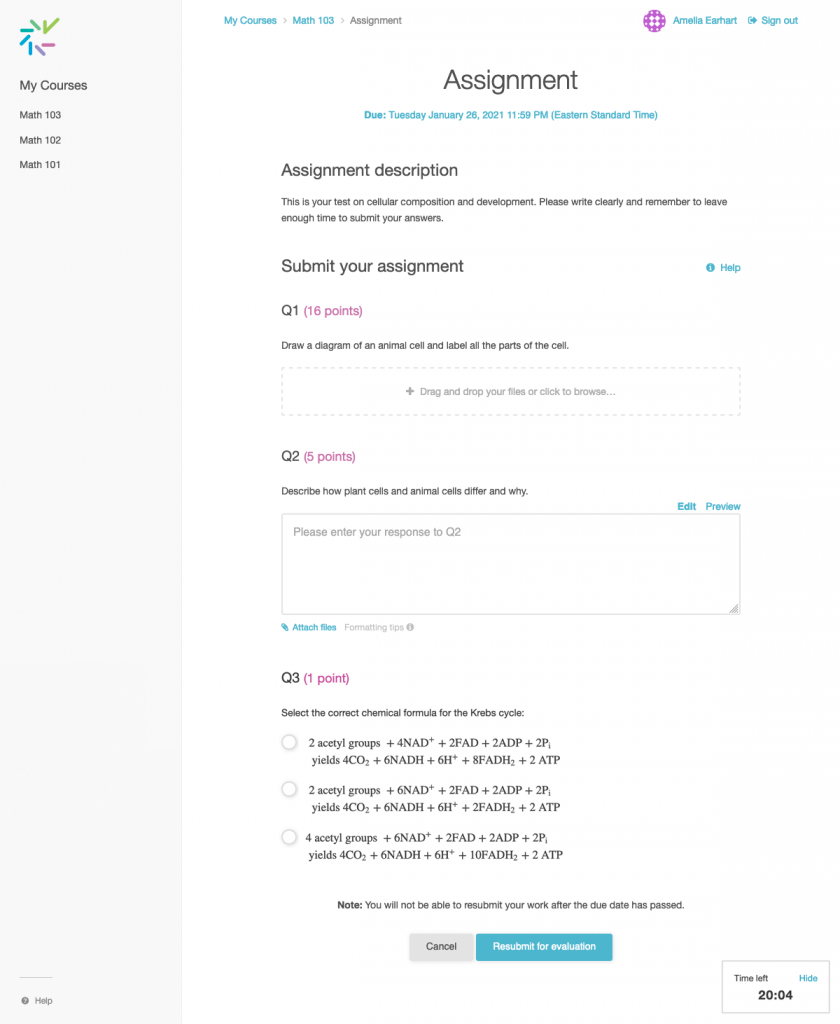
\includegraphics[alt={screenshot of assignment page on Crowdmark},width=.6\textwidth]{Day01-Crowdmark.png}

\end{frame}
%--- Next Frame ---%
\begin{frame}[c]{Office hours}
\centering
\bvfill
%Zoom link: Look up on \href{https://msu-cmse-courses.github.io/CMSE381-F25/Course_Info/Schedule.html\#google-calendar-for-office-hours}{calendar on the website}
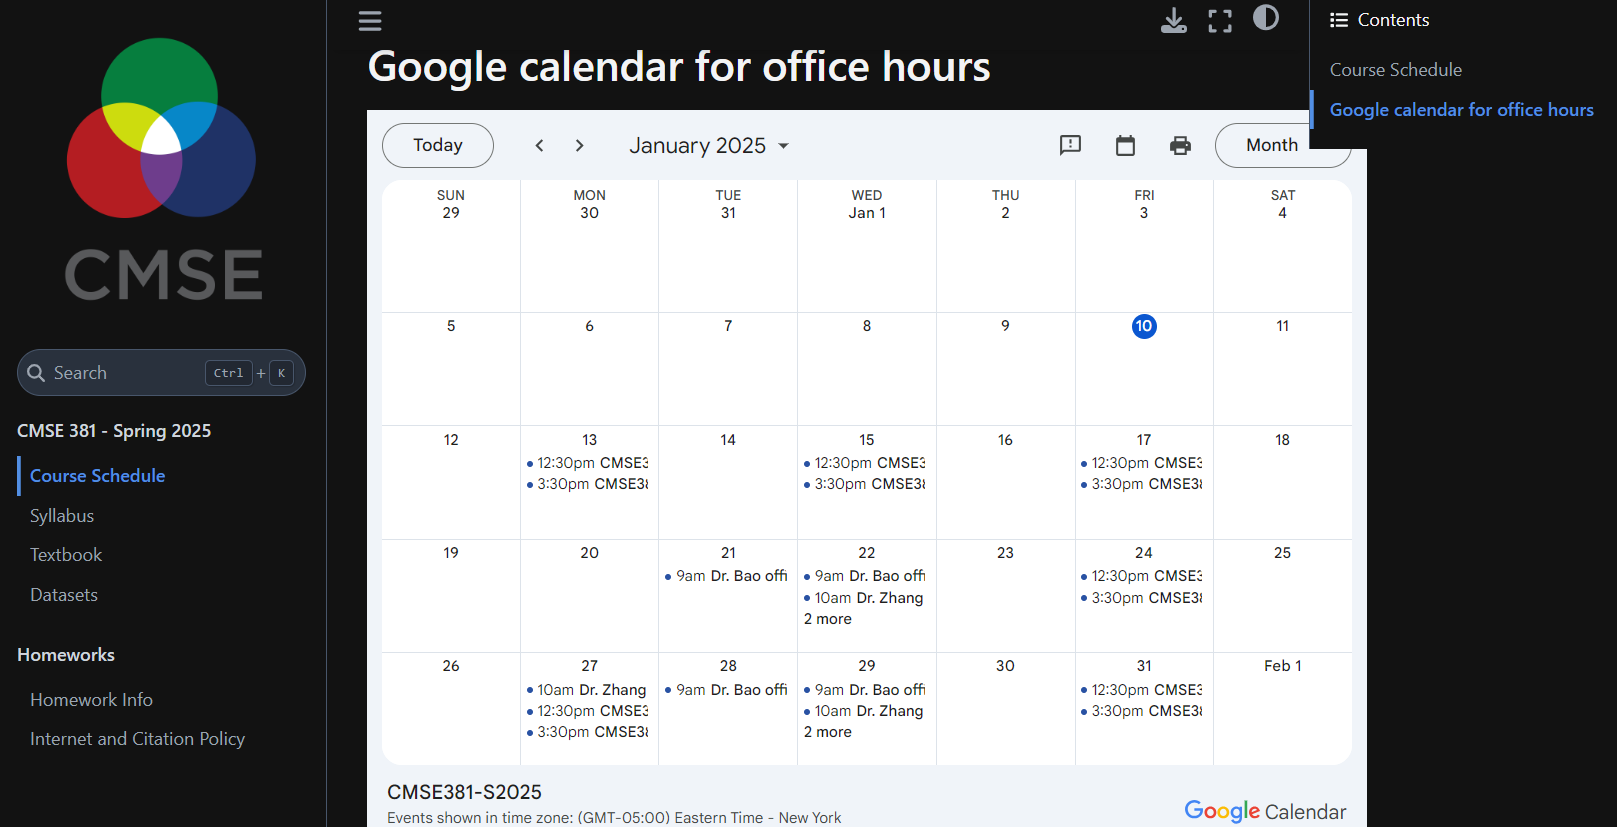
\includegraphics[alt={screenshot of Google calendar with office hours},width=.6\textwidth]{googlecalendar_s25_001.png}

\bvfill
\begin{columns}
\column{.4\textwidth}
\centering
\textit{Dr. Bao}

 \vspace{.1in}

 Time: Tues 9 am - 11 pm \\
 (Starting 1/20)


 \vspace{.1in}
 In-person (EB 2507L)


\column{.4\textwidth}
\centering
\textit{Siyu Guo
}
 \vspace{.05in}

 Time: Tue/Thu 3-4pm

%  \vspace{.1in}
 In-person (EB 2504)
% Tuesdays 2-4pm\\
% Fridays 12-2pm 



\end{columns}

\bvfill
\end{frame}
%--- Next Frame ---%
\begin{frame}[c]{Textbook}

	\begin{columns}
		\column{.4\textwidth}
	\textbf{Free download} \url{https://www.statlearning.com/}

		\column{.25\textwidth}
	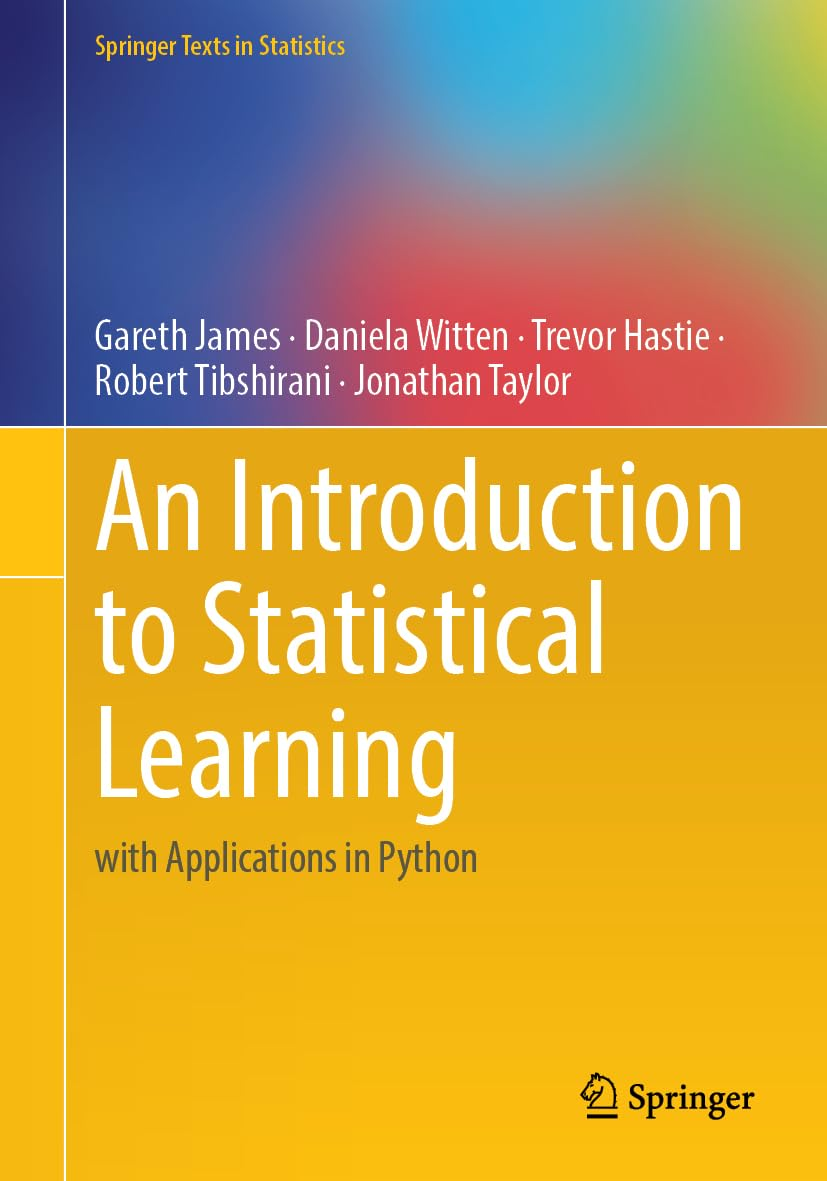
\includegraphics[alt={screenshot of the course textbook},width = \textwidth]{Day01-TextbookScreenshot}
	\end{columns}

\end{frame}
%--- Next Frame ---%
\begin{frame}[c]{Class Structure}
\begin{itemize}
	\item Class is a combination of lecture time, and group work/coding time.
	\begin{itemize} 
		\item Bring computer every day 
		\item Jupyter notebooks
		\item Python
	\end{itemize}
	\item Once a week, there will be a short check-in quiz. This will be basic content realted to lectures since the last class. Possible questions include checking on definitions, or basic understanding of major ideas.
	\begin{itemize}
		\item 10 points per quiz
		\item Drop two lowest grades
	\end{itemize}
	
\end{itemize}
\end{frame}
%--- Next Frame ---%



%--- Next Frame ---%
\begin{frame}[c]{Class Structure Pt 2}
	\begin{itemize}
		\item Homeworks due once a week, midnight of the day marked in the schedule (mostly Sundays).
		\begin{itemize}
			\item 20 points per homework 
			\item Drop two lowest grades 
			\item Sliding scale: 
			\begin{itemize}
				\item 24 hours late: 5\% penalty.
				\item 48 hours late: 15\% penalty.
				\item $>$48 hours: No late work accepted.
			\end{itemize}
		\end{itemize}
		\item Three Midterms
		\begin{itemize}
			\item See schedule for dates 
			\item 100 points each 
			\item Not cumulative 
		\end{itemize}
		\item One Project 
		\begin{itemize}
			\item Analyze dataset using tools in class, submit written report
			\item 100 points 
			\item Due at the end of the semester
		\end{itemize}
	\end{itemize}
\end{frame}

%--- Next Frame ---%
\begin{frame}[c]{Basic Expectations}
	\begin{itemize}
		\item attend each class for the full 70 min duration
		\item take detailed notes on, or beside, the skeleton slides provided.
		\item complete the jupyter notebook in class. 
		\item read the assigned textbook chapters listed in the course schedule (on course website).
		\item actively participate in group work and interactive Q\&A sessions.
		\item complete all homework assignments, quizzes, exams, and a semester project. 
	\end{itemize}

\end{frame}

%--- Next Frame ---%


\begin{frame}[c]{Approximate schedule}
	\framesubtitle{Up to date version: \url{https://msu-cmse-courses.github.io/CMSE381-S26/Course_Info/Schedule.html}}

\begin{columns}
\column{.32\textwidth}

\includegraphics[alt={screenshot of course class schedule for lectures 1 to 12},width = \textwidth]{../Figures/Schedule-S26-1}
\column{.32\textwidth}
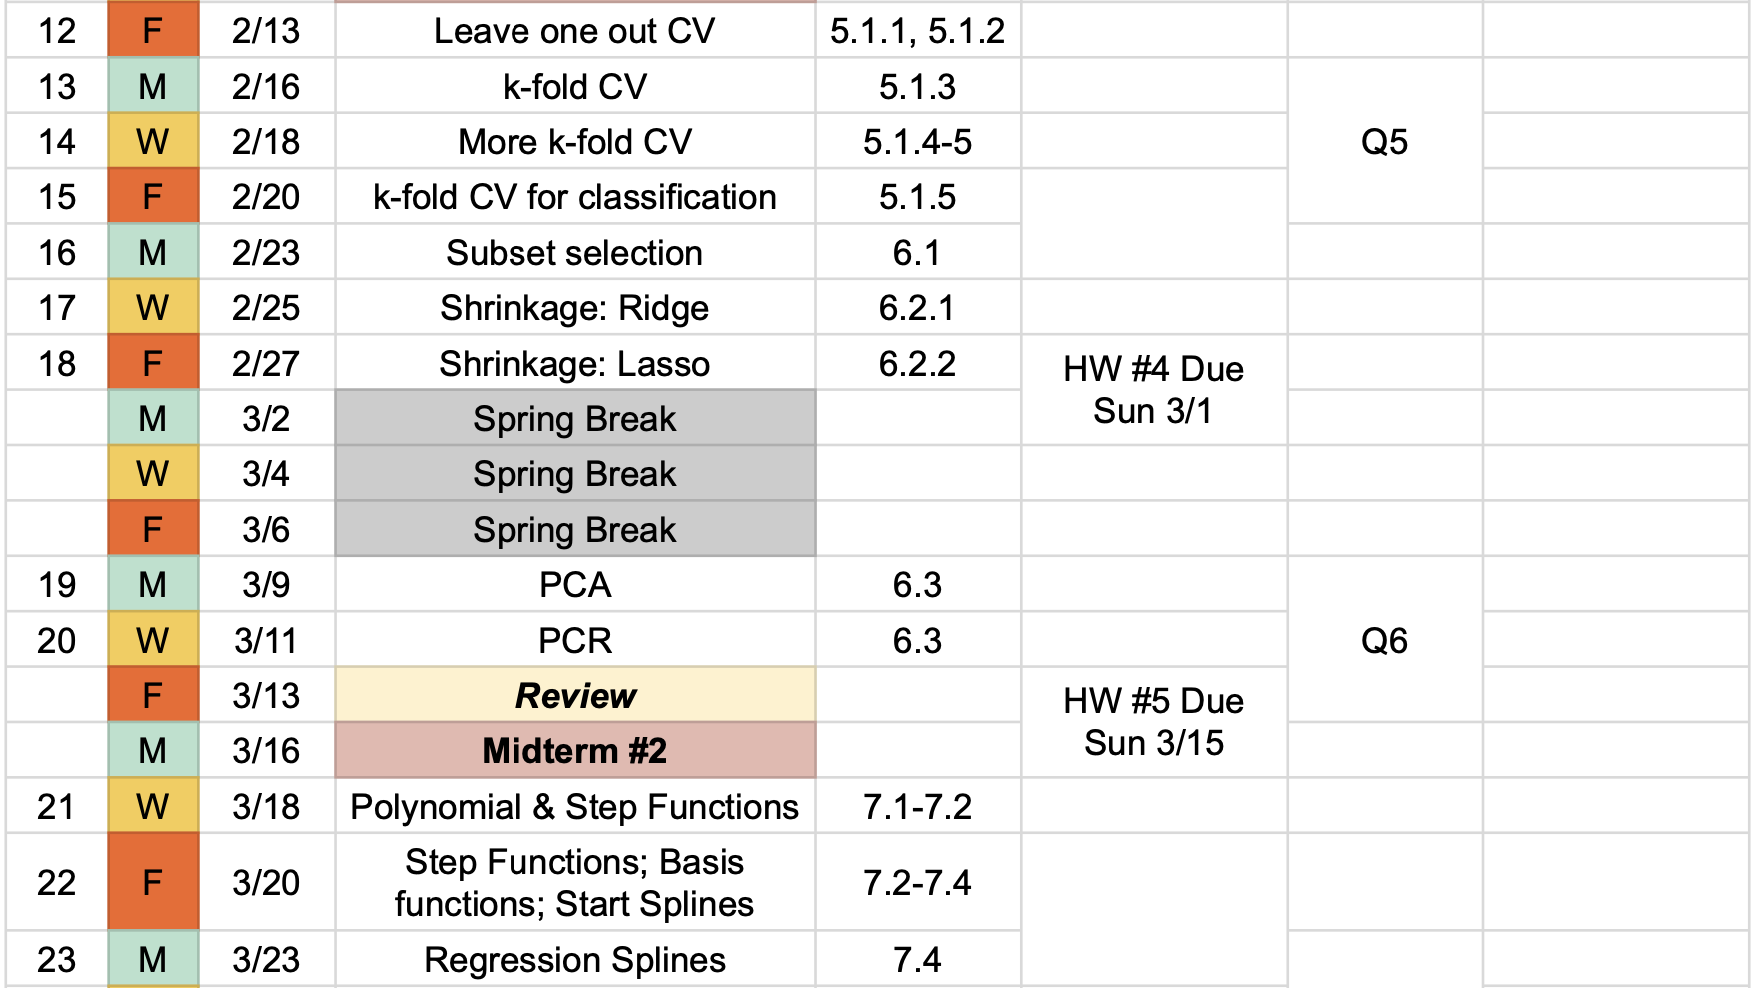
\includegraphics[alt={screenshot of course class schedule for lectures 12 to 23},width = \textwidth]{../Figures/Schedule-S26-2}
\column{.32\textwidth}
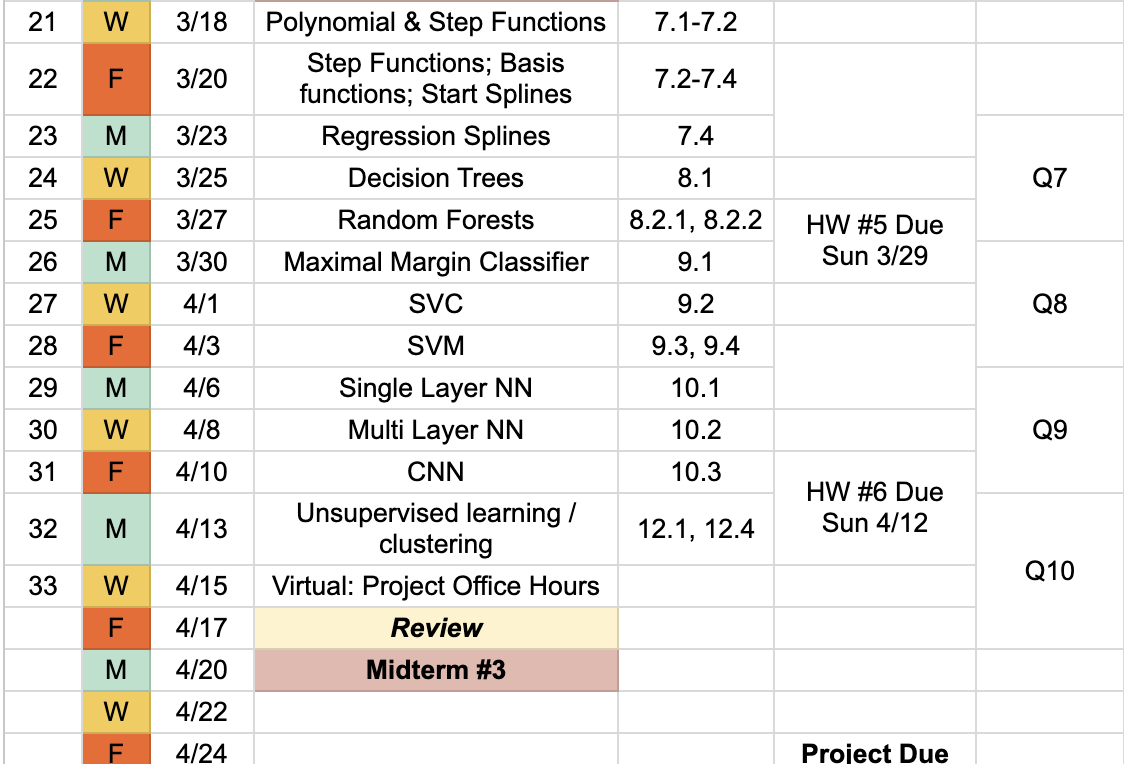
\includegraphics[alt={screenshot of course class schedule for lectures 23 to 32},width = \textwidth]{../Figures/Schedule-S26-3}
\end{columns}

\end{frame}
%--- Next Frame ---%
\begin{frame}[c]{Grade distribution}
	\centering
\begin{tabular}{lc}
&\textit{Estimated Points}\\
Homeworks & (9 homeworks - 2 lowest grades) $\times$ 20 points $=$ 140  \\
Quizzes & (10 Quizzes - 2 lowest grades) $\times$ 10 points $=$ 80\\
Midterm & (3 Midterms) $\times$ 100 $=$ 300 \\
Final Project & 100 \\
\hline
TOTAL: & 620 (Subject to change!)
\end{tabular}
\end{frame}


%--- Next Frame ---%
%=====================
\section{Intro to class}
%=====================

% \begin{frame}[c]{What is machine learning}
%
% \begin{columns}
% \column{.4\textwidth}
% Arthur Samuel (1959, IBM): Field of study that gives computers the ability to learn without being explicitly programmed
% \column{.4\textwidth}
% [add fig from yuying's slide 14]
% \end{columns}
%
% \end{frame}
%--- Next Frame ---%
\begin{frame}{What is Statistical Learning?}


	\bvfill
	\begin{columns}
	\column{.5\textwidth}
	\centering
\textbf{Statistical Learning}
\begin{itemize}
	\item Subfield of statistics
	\item Emphasizes models and their interpretability, precision, and uncertainty
\end{itemize}

	\column{.5\textwidth}
	\centering
	\textbf{Machine Learning }

	\begin{itemize}
\item
Machine learning has a greater emphasis on large scale applications and prediction accuracy.
	\end{itemize}
	\end{columns}

	\bvfill \centering

	\textit{Nowadays....to sound pedantic or techie?}
	\bvfill

\end{frame}
%--- Next Frame ---%
\begin{frame}[c]{Why should you care?}

\begin{columns}
\column{.4\textwidth}

Data is everywhere, getting more complicated and useful. Learning how to analyze data is critical.
\begin{itemize}
	\item
Web data, e-commerce (Amazon, JD, Alibaba)
	\item
Car sales (Tesla, Ford, and GM)
	\item
Sports team (MSU, Lions, etc)
\item Politics and government
\item Image, videos, text
\item even fancier data in biomedicine

\end{itemize}
\column{.4\textwidth}


% Interpreting results and prevent any bad decisions.

\end{columns}

\end{frame}
%--- Next Frame ---%
\begin{frame}[t]{Learning Tools as Black Boxes? Or Math Apocalypse?}

	\begin{itemize}
		\item Need to understand the machinery enough to
		\begin{itemize}
			\item know what tool to use
			\item know how to interpret output of the tool
		\end{itemize}
		\item Don't need to rebuild the entire box from scratch
	\end{itemize}
\end{frame}
%--- Next Frame ---%
\begin{frame}[t]{Example: Email spam }
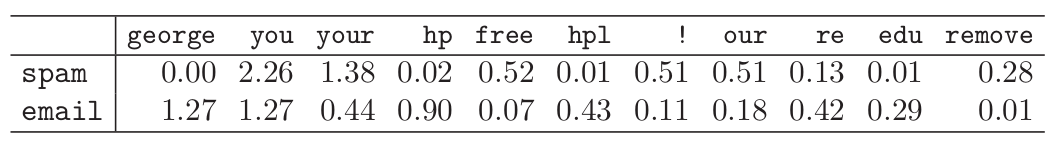
\includegraphics[alt={table of distribution of strings in samples of spam versus non-spam emails},width = \textwidth]{ESLR-Table1-1.png}
% Average percentage of words or characters in an email message equal to the indicated word or character. We have chosen the words and characters showing the largest difference between spam and email.
\begin{columns}
\column{.45\textwidth}
\centering
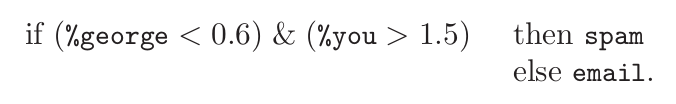
\includegraphics[alt={Example if statement to determine whether an email is spam or not},width = \textwidth]{ESLR-Table1-1-Rule1.png}
\column{.45\textwidth}
\centering
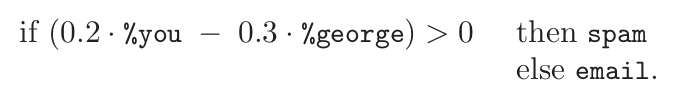
\includegraphics[alt={Example if statement to determine whether an email is spam or not},width = \textwidth]{ESLR-Table1-1-Rule2.png}

\end{columns}

\end{frame}
%--- Next Frame ---%
% \begin{frame}[c]{MNIST}
% 	% \centering
% 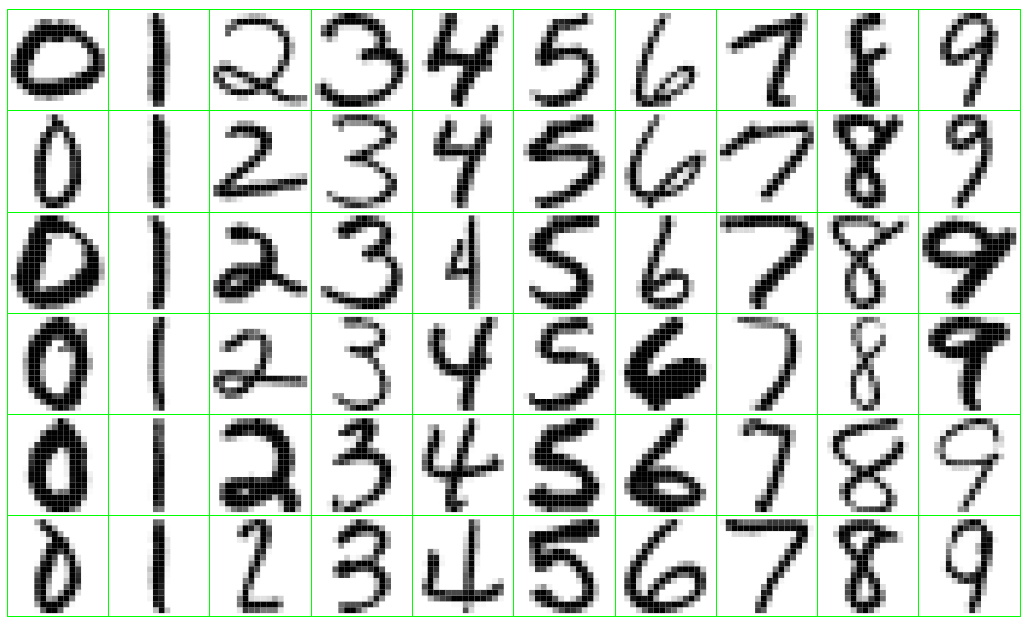
\includegraphics[width = .4\textwidth]{ESLR-Fig1-2.png}

% \end{frame}
%--- Next Frame ---%

\begin{frame}[c]{Supervised learning}

\begin{itemize}
	\item Outcome measurement $Y$ (also called dependent variable, response, target, label).

\item
Vector of $p$ predictor measurements $X$ (also called inputs, regressors, covariates, features, independent variables).

\item
In the regression problem, $Y$ is quantitative (e.g price, blood pressure).

\item
In the classification problem, $Y$ takes values in a set of distinct categories (survived/died, cancer class of tissue sample, types of language).
\end{itemize}
\begin{columns}
\column{.4\textwidth}
\centering

\column{.4\textwidth}
\centering

\end{columns}

\end{frame}
%--- Next Frame ---%

\begin{frame}[c]{Unsupervised learning }

\begin{itemize}
	\item
No outcome variable, just a set of predictors (features) measured on a set of samples.

	\item
Objective is fuzzier: often explore the intrinsic relation between samples (e.g.,clustering) or features (e.g. dimensionality reduction)
% find groups of samples that behave similarly, find features that behave similarly, find linear combinations of features with the most variation.

	\item
Difficult to know how well you are are doing

	\item
Different from supervised learning but can be useful as a pre-processing step for supervised learning.
\end{itemize}

\end{frame}
%--- Next Frame ---%
{
\setbeamercolor{background canvas}{bg=Apricot!25}
\begin{frame}[t]{Generative AI discussion}
\begin{columns}
\column{.5\textwidth}
Definition via \href{https://en.wikipedia.org/wiki/Generative_artificial_intelligence}{Wikipedia}:\\ 
\begin{quote}
	Generative artificial intelligence (AI) is artificial intelligence capable of generating text, images, or other media, using generative models.
	Generative AI models learn the patterns and structure of their input training data and then generate new data that has similar characteristics.
\end{quote}

Examples:
\begin{itemize}
	\item ChatGPT
	\item Bard
	\item DALL-E
\end{itemize}
\column{.49\textwidth}
\centering
\begin{itemize}
	\item Get in a group of about 4. 
	\item Open this google doc: \href{https://tinyurl.com/CMSE381-S26-genAI}{tinyurl.com/CMSE381-S26-genAI}
	\item In your group, brainstorm cases where someone might use generative AI in the context of our class. 
	\item Once you have added a few, start adding arguments for or against whether we should allow the use of that context in class. 
\end{itemize}
\end{columns}
\end{frame}
}
%--- Next Frame ---%



\section{Python Review Lab: Pt 1}

%--- Next Frame ---%
{
\setbeamercolor{background canvas}{bg=Apricot!25}
\begin{frame}[t]{Plan for the lab}
\begin{columns}
\column{.8\textwidth}
\centering
\begin{itemize}
	\item Find a group of 4 or so. 
	\item Find the class website (\href{http://cmse.msu.edu/CMSE381}{cmse.msu.edu/CMSE381}) or (\href{https://msu-cmse-courses.github.io/CMSE381-S26/}{msu-cmse-courses.github.io/CMSE381-S26/}) and download the jupyter notebook for the Python Review Lab.
	\item Get started!
\end{itemize}

\vspace{.2in}


\includegraphics[alt={screenshot of lecture 1 Jupyter notebook},width = .8\textwidth]{Day01-Website-FirstNotebook-Screenshot}
% \textbf{Using git}
% \begin{itemize}
% 	\item \texttt{git clone git@github.com:msu-cmse-courses/cmse381-F23.git}
% 	\item from inside the folder you just made, run \texttt{git pull} any time you want to download new content
% \end{itemize}

% \column{.45\textwidth}
\centering
\end{columns}
\end{frame}
}
%--- Next Frame ---%

% \begin{frame}[c]{Data Ethics}
% \begin{itemize}
% 	\item Data affects people
% 	\item Your decisions on how to analyze and interpret data matter
% \end{itemize}


% \end{frame}
%--- Next Frame ---%


%
% \begin{frame}[t]{Example: Presidential election}
% 	PIC OF NATE SILVER
%
% 	On 2008, he correctly predicted the winner of 49 of the 50 states and all 35 U.S. Senate races .
% On 2012, he correctly predicted the winner of all 50 states and the District of Columbia.  That same year, Silver's predictions of U.S. Senate races were correct in 31 of 33 states.
% All the data he used came from internet!
% Dow down 313 points after Obama won
% \end{frame}
% %--- Next Frame ---%
% \begin{frame}[c]{Supervised Learning}
%
% \begin{columns}
% \column{.4\textwidth}
%
% \column{.4\textwidth}
%
% \end{columns}
%
% \end{frame}
% %--- Next Frame ---%
% \begin{frame}[c]{Unsupervised learning}
%
% \begin{columns}
% \column{.4\textwidth}
%
% \column{.4\textwidth}
%
% \end{columns}
%
% \end{frame}
% %--- Next Frame ---%

% %----------------
\begin{frame}[c]{Next time}

\begin{columns}
\column{.5\textwidth}
\centering
	\begin{itemize}
		\item Weds: What is statistical learning? (Reading 2.1)
		%\item No class coming Monday (9/1)
		\item First HW Due Sunday, 1/25
		\item Quiz sometime \textbf{this} week
		\item Office hours: 
		\begin{itemize}
			\item Most up-to-date on the website
			\item Starting next week
		\end{itemize}
	\end{itemize}

\column{.4\textwidth}
\centering
\includegraphics[alt={screenshot of course class schedule for lectures 1 to 12},align = c, width = \textwidth, trim = 0 100 0 0, clip]{Schedule-S26-1.png}


\end{columns}
\end{frame}
%--- Next Frame ---%


\end{document}
